%This chapter presents the context, motivation and PhD framework railways WSN-based smart grid. 

\section{Context and motivation of PhD}

The railway system is responsible for 1.3\% of entire European energy consumption, \cite{iea-uic2016}. 
The debate on energy efficiency in railways is a well-discussed topic due to its impact on the global energy consumption.

The energy efficiency analysis and management requires a detailed mapping of the energy consumption/generation in the railway system. 
This detailed mapping of the energy flows should include, not only the rolling stock level but also the traction substations and the auxiliary services.
The knowledge of all the load curves permits load prevision, peak shaving and energy cost optimization for the entirely of the railway system.


\section{Shift2Rail Framework}

This work is supported by the iRail PhD programme – Innovation in Railway Systems and Technologies whose objectives are aligned with the \ac{S2R} objectives, \cite{shift2rail2015}, which are: 

\begin{itemize}
	\setlength\itemsep{-0.5em}
	\item 1. Cutting the life-cycle cost of railway transport by, at least, 50\%;
	\item 2. Doubling the railway capacity;
	\item 3. Increasing the reliability and punctuality by 50\%, at least.
\end{itemize}

Complementary, the time target goals are the establishment of a framework, by 2020, for a European multimodal transport system for the passenger rail, freight and for the urban mobility. By 2030 is expected to triple the length of the existing high-speed passenger rail network, 30\% of the road freight over 300 km should shift to rail or waterborne transport and achieve a CO2-free city logistics in major urban centers. By 2050, the medium-distance passenger transport should go by rail and hight-speed rail, with the connection of all core network airports to the high-speed railway network. On the freight is expected to have all seaports connected to the rail freight transport system and on the urban mobility, the "conventionally-fueled" cars will not have place in cities by 2050, \cite{shift2rail2015}.


The \ac{S2R} carries five innovation programmes, as presented in figure \ref{fig:ips}. Framed on the S2R \ac{IP3} with the focus on the ”Cost efficient and reliable infrastructure”, it is proposed the development of a \ac{SMD} that achieves a detailed monitoring and supervision of various energy flows on the premises of embracing the entire \ac{RTS}.

\begin{figure}[h!]
	\centering
	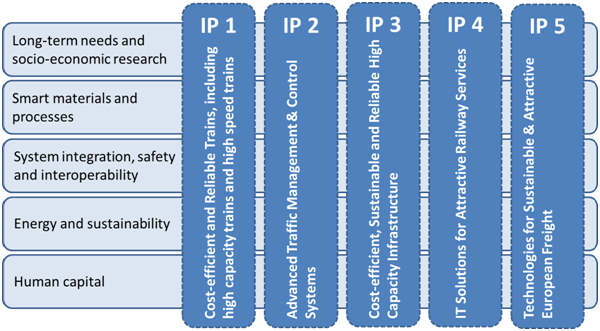
\includegraphics[width=0.60\textwidth,keepaspectratio]{figures/1.Intro/IPs}
	\caption{Shif2Rail Innovation Programs. }
	\label{fig:ips}
\end{figure}

The purpose of any energy management strategy is to build the dynamics of every loads and generators of the power system. 
This should be performed based on an extensive knowledge of every energy flows. 
This way, the \ac{SMD} is required to propose and validate a standard metering architecture that involves the coordination of every measurements either in on-board and in ground. 
In advance, energy data analysis should be provided based on relevant stored data. 

\section{Preliminary state of the art}

This section will cover a summary of the state of the art that supports this PhD.

Based on the state of the art, current metering systems focus on rolling stock on-board energy meters for energy billing purposes only, being located close to the pantograph, \cite{shift2rail2015}.
A possible advancement beyond the state of the art is the expansion of the measurement system at railway system level, making it a distributed on-board and track-side measurements, thus achieving detailed mappings. 

%\vspace{2em}

Other issue shown in the state of the art is the intrusion level of currently used metering systems, that in a way, became a critical subsystem of the rolling stock but also requires a relatively long implementation, \cite{shift2rail2015}. 
An advance beyond the state of the art is a solution based on non-intrusive technology. More detailed simulation models in conjunction with field measurements is included on the methodology to be investigated.



%\textbf{\textit{Research Plan}}

A specific challenge and requirements of this research is the development of non-intrusive  \ac{WSN}  in the railway environment. 
It is intended that this technology should be based on an open system and open interfaces for the data collection, aggregation and analysis. 
Issues like metering redundancy, outlier detection, fault tolerance and communication reliability, should be considered during the research.
In addition, it is expected the design and specification of a set of user applications.
Those applications are focused in the energy analysis process, with the aim of providing more information and detailed knowledge.
This detailed knowledge will be useful in a decision support system related with, in e.g., eco-driving strategies, timetable planning and preventive maintenance.

\newpage

\section{Document structure}

This document is divided in 5 chapters, each of them incorporating the relevant subsections to present the subjects mentioned. 
%contains several subsections according to the subjects mentioned.

\begin{table}[!h]
	\label{tb:struct}
	\centering
	\caption{Document structure}
	\vspace{0.2em}
	\begin{tabular}{c|l}%{C{2cm}|C{9cm}}
		\textbf{Chapter} & \textbf{Title}                    \\ \hline
		1       &                   Introduction             \\ \hline
		%  2       &                   Railways Remote Monitoring Systems       \\ \hline
		2       &                   Objectives and Contributions    \\ \hline
		3       &                   Literature Review    \\ \hline
		4       &                   Methodology and Work Plan       \\ \hline
		5       &                   Preliminary Work       \\
	\end{tabular}
\end{table}